\chapter{Literature Review}
\label{cha:Literature Review}

\section{Car Following Models}
\label{sec:Car Following Models}
Any autonomous-vehicle system will implement a `car-following model', which defines actions for a vehicle based on the behaviour of its predecessors (the vehicles in front of it). One early car-following model was defined in 1981 by P.G. Gipps \citep{Gipps1981}. It was designed to mimic real-world driver behaviour, calculating a safe travelling speed for a vehicle based on the speed of its predecessor. A safe travel speed is defined as a speed at which the driver can safely stop if the preceding driver stops.

Gipps defined two equations applying constraints on the acceleration and braking profiles of the vehicles. Appendix \ref{subsec:Gipps 1981 Equations} details these equations. Gipps' model worked well at describing the behaviour of traffic. However, translating this work to autonomous vehicles poses a number of problems. Firstly, the work is based on the behaviour of real-world drivers in instrumented vehicles. This introduces human driver variables into the equations. Gipps' modelled reaction time, which will be far smaller for autonomous vehicles. The gaps between successive vehicles are also larger than necessary. Autonomous vehicles are more precise than human drivers and can drive closer to their predecessors. Gipp's model also focuses solely on single-lane drivers.

In 2000 Treiber et al. suggested the `Intelligent Driver Model' (IDM) \citep{Treiber2000}. This model, detailed further in Appendix \ref{subsec:The Intelligent Driver Model}, defines an acceleration profile for a vehicle as a continuous function. This function is based on the vehicle's current velocity, its desired velocity and the distance from the vehicle to its successor.

The IDM does not attempt to directly mimic human behaviour in traffic situations. It models a general acceleration and braking profile for a given vehicle. As such, it is well suited for adaptation by autonomous vehicle models, as seen in Kesting's work \citep{Kesting2007} in Section \ref{subsec:Lane Changing to improve overall velocity}. However, similarly to Gipps' model, it solely focuses on single-lane drivers.

Gipps' model and the IDM also both fail to recognise, and incorporate, the use of vehicle-to-vehicle communication in their models. Autonomous vehicles could communicate with each other to help reduce overall travel time and improve efficiency. In vehicle platoons, such as those analysed by Kamali in 2016 \citep{Kamali2016}, each vehicle autonomously follows it's predecessor, with the lead vehicle controlling the overall pace of the platoon. Platoons make heavy use of vehicle-to-vehicle (V2V) communication to allow vehicles to join and leave, as well as to continuously control vehicle spacing and velocity. The advantage of a platoon is that all vehicles can accelerate and decelerate simultaneously reducing the effect of traffic shocks \citep{Daganzo1994}.

\section{Centralised and Decentralised}
\label{sec:Centralised and Decentralised}
We can divide approaches to autonomous vehicles into centralised and decentralised solutions. Centralised solutions rely on an external agent to manage vehicles. Vehicles use vehicle-to-infrastructure (V2I) communication channels to send information and receive instructions from the external agent. Decentralised solutions use vehicle-to-vehicle (V2V) communication to let other vehicles know their state, their intentions and to arrange any complex actions that might affect surrounding vehicles.

\subsection{Centralised Systems}
\label{subsec:Centralised Systems}
The Autonomous Intersection management system (AIM) described in \citep{Dresner2004} is an example of a centralised V2I system. The system works by dividing the intersection into a grid of $n \times n$ reservation tiles. Drivers `call ahead' to the intersection sending information packets containing

\begin{enumerate}
\item The time the vehicle will arrive.
\item The velocity at which the vehicle will arrive
\item The direction the vehicle will be facing when it arrives
\item The vehicle's maximum velocity
\item The vehicle's maximum and minimum acceleration
\item The vehicle's length and width
\end{enumerate}

The intersection infrastructure simulates the journey of the vehicle through the intersection, noting the tiles occupied by the vehicle at each time interval. If any cell is reserved at the same time step the intersection rejects the request. The driver will start decelerating and continue making requests until it obtains a reservation. It will not enter the intersection without a reservation, even if that means coming to a stop at the intersection.

\begin{figure}[htb]
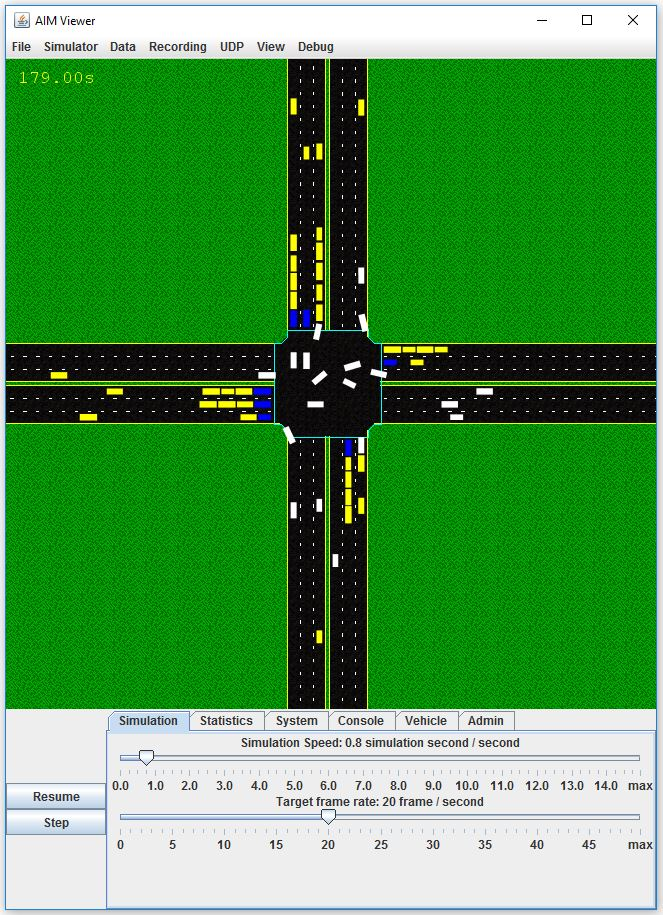
\includegraphics[width=\textwidth]{litReview/aimOriginal.JPG}
\caption{Screenshot of the AIM Simulator}
\label{fig:AIMOriginal}
\end{figure}

A grid-based reservation system works well in high traffic zones like intersections, because it forces all vehicles to communicate with a single entity. This entity has a global-view of activity at the junction, allowing the system to make vehicle management decisions more easily. A V2V solution would require more complex communication protocols involving large numbers of vehicles. The volume of messages required for each vehicle to obtain a global view of the intersection would be considerably larger, and as such, most vehicles will never get a complete understanding of the status of the intersection.

This paper forms the foundation for the AMM protocol designed in Section \ref{sec:Autonomous Merge Management System}.

\FloatBarrier
\subsection{Decentralised Systems}
\label{subsec:Decentralised Systems}
The main arguments against centralised systems generally tend to stem from concerns over feasibility and fault tolerance. A centralised V2I solution relies on one system always being available to manage vehicles. The original implementation of the AIM system works well, but if the system were to fail and no longer provide reservations, then approaching vehicles will simply halt at the intersection. In a worst case scenario, the system would still give reservations, but fail to compare them to reservations already in place, causing major car crashes in the intersection. Having, a single point of failure like this is a major concern, particularly when lives are on the line.

A paper by VanMiddlesworth et al. in 2008 \citep{VanMiddlesworth2008} defined a decentralised version of the AIM model using V2V communication protocols. In VanMiddlesworth's model each vehicle can broadcast two different types of message. These messages are broadcast repeatedly with a specified period.
\begin{enumerate}
\item \emph{Claim}
This is a message indicating the vehicle's intention to traverse the intersection. It provides the vehicle's VIN, arrival lane, turning direction, arrival time and exit time. It also provides a message id, which increments when a new message is broadcast. Finally, the \emph{Claim} message contains a boolean indicating whether the vehicle has stopped at the intersection.
\item \emph{Cancel}
This message releases any currently held reservation, it contains the vehicle's VIN and a message id, which acts the same as the message id in \emph{Claim}.
\end{enumerate}

Two \emph{Claim} messages are in conflict if their paths, as determined by their lane and turn parameters, are incompatible and their time intervals, as determined by their arrival and exit times, overlap. To resolve the conflict VanMiddlesworth's model determines which Claim has dominance. A claim $C_1$ dominates another claim $C_2$ if $C_1$'s vehicle is stopped at the intersection, and $C_2$'s vehicle is not. If $C_1$ and $C_2$ both have the same value for the stopped at intersection boolean the claim has priority dominates. Priority is indicated by the following rules, in order of evaluation:
\begin{enumerate}
\item If neither vehicle is stopped at the intersection, the claim with the earliest exit time has priority.
\item If both vehicles are stopped, the vehicle whose lane is 'on the right' has priority. This is defined similarly to current US 4-way stop rules.
\item If neither lane can be considered to be on the right the vehicle who is not making a turn has priority.
\item If no other priority order can be established, the vehicle with the lowest VIN has priority.
\end{enumerate}

The protocol starts with approaching vehicles receiving messages from existing pending vehicles. An approaching vehicle may not start broadcasting it's own messages until it is within 'lurk distance' of the intersection. 

Once within lurk distance the vehicle generates a \emph{Claim} message for the earliest possible time the vehicle might arrive at the intersection. Once the vehicle has a \emph{Claim} broadcasting it may need to change it if it's looking like the vehicle might be late to the intersection or if a competing \emph{Claim} dominates it. A vehicle might also change its \emph{Claim} to take advantage of a newly available time slot. In this situation the vehicle must then send a \emph{Cancel} message and a new \emph{Claim}. The \emph{Cancel} message is sent repeatedly with the same period as the \emph{Claim} message. Once the vehicle reaches the intersection it must traverse according to its current \emph{Claim}, broadcasting its \emph{Claim} throughout the traversal. At this point, the vehicle's claim cannot be dominated.

The main drive behind the unmanaged AIM intersection was to reduce cost. Adding in new infrastructure to an intersection costs money, and it might not be considered worthwhile for small intersections with only one or two lanes on each side. An unmanaged, decentralised system like that described by VanMiddlesworth would drastically reduce the cost to the state in creating automated road networks.

This paper forms the foundation for the decentralised protocol designed in Section \ref{sec:Decentralised Merge Management System}.

\section{Making lane changing decisions}
\label{sec:Making lane changing decisions}
There are a number of reasons that a driver would want to change lanes. The most obvious being that the journey the driver wishes to complete requires the vehicle to move into a different lane. In this case the vehicle \emph{must} change lanes before it reaches a critical position. Beyond this position the driver will need to change their planned route, most likely extending their journey time. 

Another reason a driver might change lanes is in order to increase velocity, with the aim of reducing journey time. In general, a driver will aim to change lanes if their average velocity in their current lane is much less than that the velocity it could be achieving in another lane.

\subsection{Lane Changing to hit a target lane}
\label{subsec:Lane Changing to hit a target lane}
In 1986 Gipps' modelled driver behaviour in real world circumstances, characterising the decisions a driver has to make in order to determine whether to change lanes \citep{Gipps1986}. The paper was designed to be used with the Gipps' 1981 car-following model \citep{Gipps1981}, explained in \ref{sec:Car Following Models}.

The model itself is constructed as a flow chart, in which the decision nodes are the choices a driver must make.You can see the flowchart in Figure \ref{fig:Gipps1986Flowchart}.

\begin{figure}[htb]
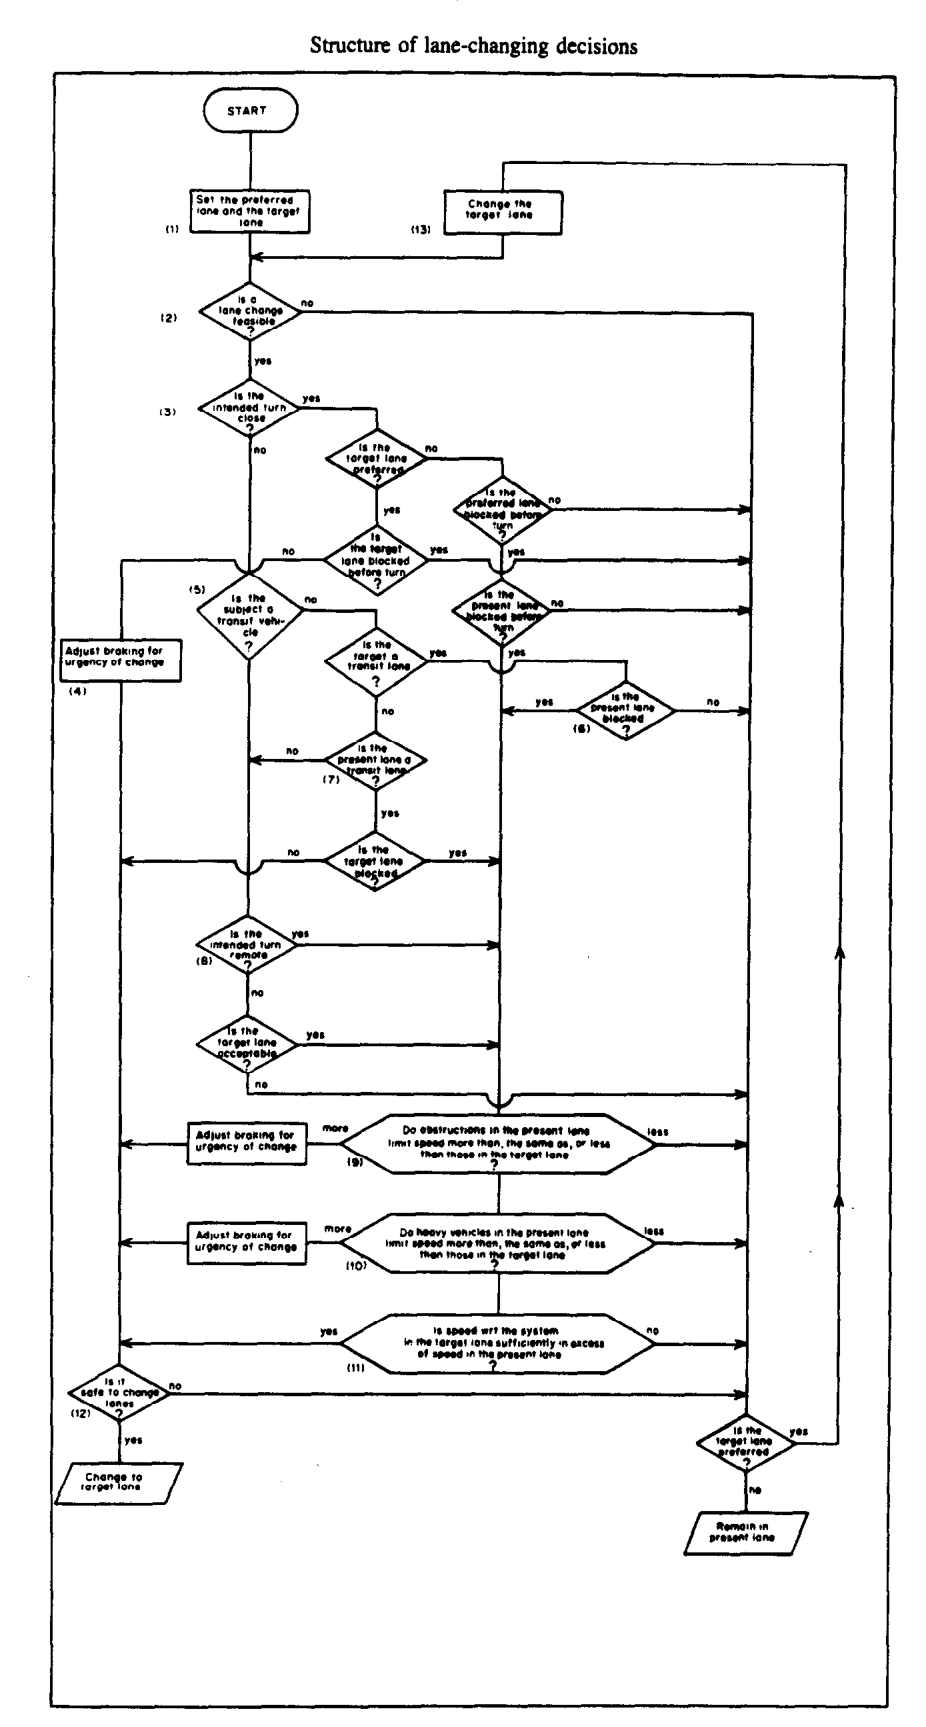
\includegraphics[width=\textwidth]{litReview/gipps1986Flowchart.png}
\caption{The flowchart for lane changing decisions from \citep{Gipps1986}}
\label{fig:Gipps1986Flowchart}
\end{figure}

After determining whether a lane change is feasible the model considers whether the driver needs to move into another lane because they are heading towards a critical point.

These decisions are modelled in nodes 3 and 4.

\begin{enumerate}
\item[3] \textit{Driver behaviour close to the intended turn}

If the driver is close to their intended turn then they will always attempt to change into their preferred lane. Only if blocked will they consider moving into another lane. 

'Close' varies depending on regional differences and the level of traffic, but in the model, close is defined as the driver being within a distance equal to ten seconds of travel from the turn at the driver's desired speed.

\item[4] \textit{Urgency of changing lanes}

The urgency of changing lanes increases as the driver gets closer to their turn. The willingness of the driver to brake harder and accept smaller gaps increases as the driver gets closer to their intended turn.

In the implementation, the braking rate a driver is willing to when first becoming close doubles by the time the intended turn is reached. 

\begin{itemize}
\item[$D_n$] is the location of the intended turn
\item[$V_n$] is the desired (or free) speed of the driver
\item[$b_n^*$] is the most severe braking the driver would otherwise be willing to undertake
\end{itemize}

\begin{equation}
b_n = \Biggl[2 - V_n\frac{(D_n - x_n(t))}{10}\Biggr]b_n^*
\end{equation}

\end{enumerate}

Similarly to Gipps 1981 car-following model, this driver decision model is based on human driver behaviour and as such falls into similar pitfalls. There could be more optimal driver behaviours which would ensure that a driver is in the correct lane well before the critical position. However, because Gipps 1986 model is designed to model human driving behaviour we can expect it to perform less than optimally.

Atagoziyev's model is designed around autonomous vehicles, which allows it to take advantage of vehicle-to-vehicle communication. The model manages a set of vehicles over two lanes, organising their movements into their preferred lanes before they reach a critical position.

To do this the model keeps track of the gaps between vehicles and their relative speeds using roadside infrastructure. Then, a series of equations, each describing a different situation, are used to determine the behaviour of the vehicle.

In the paper SV (subject vehicle) refers to the vehicle that wants to change lanes. CL (current lane) is the vehicle in front of the SV. TL (target lane) is the vehicle the SV wants to be behind in its target lane. LV (lag vehicle) is the vehicle that will be behind SV once it moves to its target  lane. Atagoziyev defines seven equations for manipulating vehicles between lanes. They are used in different contexts, each based on the relative positions of the surrounding vehicles. The contexts for each equation are given below, along with the behaviour from the equation during that context.

\begin{enumerate}
\item[Case 1] \textit{SV too close to CL in its current lane or TL if it changed lanes.}

SV slows down until the gap is sufficiently large enough.
\item[Case 2] \textit{SV has a large gap between itself and TL and CL, however, LV is too close to SV}

SV can approach CL and TL as long as the gap remains large enough. LV needs to open up a sufficient gap behind SV.
\item[Case 3] \textit{SV has the minimum allowable gap to TL and CL, but LV is too close}

SV follows the closest leader and waits until LV creates the necessary gap.
\item[Case 4] \textit{The gaps between SV and CL/TL/LV are sufficient. But CL/TL are not travelling at the 'nominal speed' established for all vehicles in this exchange}

SV maintains a sufficient gap, waiting for CL/TL to travel at nominal speed again.
\item[Case 5] \textit{SV and CL/TL/LV have sufficient gaps and CL/TL are travelling at nominal speed.}

SV performs the lane change, maintaining nominal speed.
\item[Case 6] \textit{SV obtains the minimum gap to CL/TL and LV maintains a sufficient gap. CL/TL are not travelling at nominal speed}

SV maintains the minimum gap, waiting for CL/TL to travel at nominal speed again.
\item[Case 7] \textit{SV obtains the minimum gap to CL/TL and LV maintains a sufficient gap. CL/TL are travelling at nominal speed}

SV performs the lane change, maintaining nominal speed.
\end{enumerate}

These equations are the building blocks that lead to a lane change. The flowchart in Figure \ref{fig:AtogoziyevFlowchart} shows how they work together to enact a single lane change.

\begin{figure}[htb]
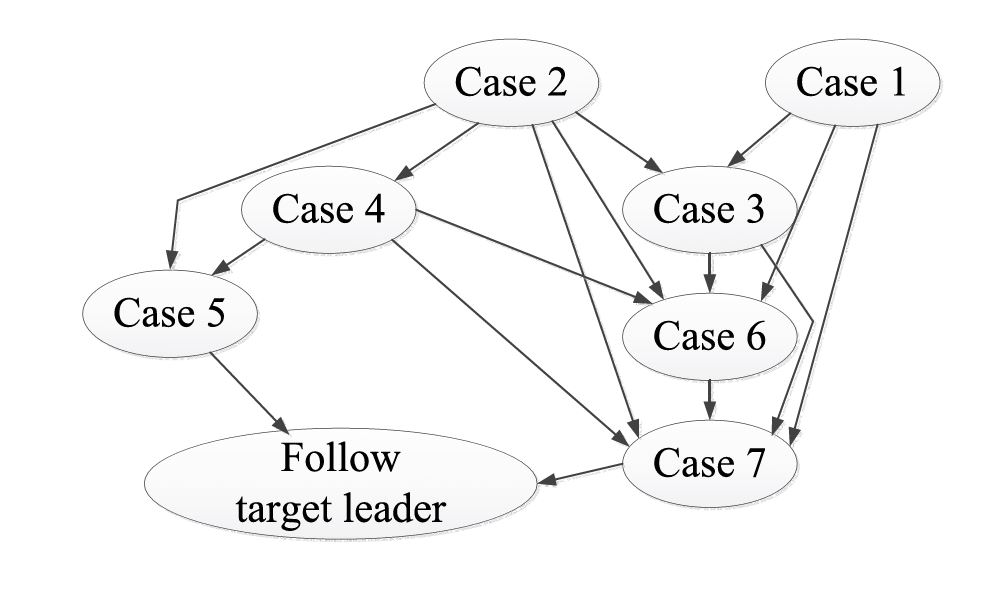
\includegraphics[width=\textwidth]{litReview/atagoziyevFlowchart.JPG}
\caption{The flowchart for Atagoziyev's Lane Changing model equations}
\label{fig:AtogoziyevFlowchart}
\end{figure}

Using this algorithm, we can move multiple vehicles into their correct lanes. LV always provides space to allow each changing vehicle into the correct lane. All of the vehicles are working with each together, such that they can all reach their goal. Comparing this to Gipps' 1986 model, where drivers are acting solely in their own interest, we can see that by having an external agent managing lane changes, the autonomous vehicles can achieve results that might not be possible in situations where drivers are acting selfishly. For example, in a grid locked situation, drivers following Gipps' model might never be able to move into their desired lane; however vehicles following Atagoziyev's model would open up spaces allowing vehicles to move through the traffic.

\subsection{Lane Changing to improve overall velocity}
\label{subsec:Lane Changing to improve overall velocity}
Gipps' driver decisions model also considered situations where the driver does not have to be in any particular lane. The model considers the effects of transit lanes, heavy vehicles and the effect of the preceding vehicle on the driver's vehicle. These are shown in nodes 5 to 7 and 9 to 11 of Gipps' flowchart in Figure \ref{fig:Gipps1986Flowchart}.

\begin{enumerate}
\item[5] \textit{Transit vehicles and lanes}
Transit lanes are lanes dedicated solely for public transport and other high occupancy vehicles. These include vehicles such as buses, taxis and carpool cars. These vehicles are known in the model as 'transit vehicles'.
\item[6] \textit{Entry of nontransit vehicles into transit lanes}
If there is an obstruction in the present lane, it is often considered to be a valid reason for a non-transit vehicle to enter a transit lane. 
\item[7] \textit{Departure of nontransit vehicles from a transit lane}
Once the obstruction has been cleared, nontransit vehicle must move back into a valid lane. This forced departure does not affect vehicles that are close to their intended turn.
\item[9] \textit{Relative advantages of present and target lanes}
If the driver has not yet been forced to change lanes by any other factors, then they can look at the relative advantages of the present and target lanes, considering obstructions and then determining which lanes obstructions will have the least effect on their safe speed.
\item[10] \textit{The effect of heavy vehicles} 
If obstructions are level with each other or beyond the range a driver considers, then the driver considers the next heavy vehicle in each lane, as if it were the leading vehicle in an ordinary car following situation. The driver then selects the lane which will give them the higher speed.
\item[11] \textit{The effect of the preceding vehicle}
If there are then no heavy vehicles, the driver considers the speed possible in each lane and then changes if they gain a 'sufficient' speed advantage. This is again, subjective, depending on the present lane, target lane and the type of vehicle.
\end{enumerate}

Again, Gipps' 1986 model was built with human drivers in mind, and as such it fails to take advantage of the benefits of autonomous vehicles such as platooning and vehicle-to-vehicle communications.

Work by Kesting et al. in 2007 \citep{Kesting2007} describes a decentralised model of lane changing that lets vehicles change lanes to increase velocity whilst still ensuring that the overall traffic flow is not disrupted. This helps to avoid traffic shocks and maintains smooth traffic flow. In order to do this, Kesting introduces the MOBIL or 'Minimising Overall Braking Induced by Lane Changes' model. The model uses two criterion that the vehicle must satisfy.

The first criterion deals with safety, ensuring that the deceleration of a successor vehicle $\tilde{a}_n$ in the target lane doesn't exceed a safety limit $b_{safe}$.

\begin{equation}
\tilde{a}_n \geq -b_{safe}
\end{equation}

This criterion effectively puts a limit on the level of braking a vehicle changing lanes can cause another vehicle to undergo if it pulls out in front of it.

The second criterion is the 'incentive criterion' which is what motivates a driver to change lanes. This criterion introduces a 'politeness factor' $p$ which expresses the extent to which nearby vehicles affect a driver's lane changing decision. 

The paper discusses the differences between symmetric ('US') lane changing rules and asymmetric ('European') passing rules, however in this paper we only use US lane changing rules. This gives the incentive criterion:

\begin{equation}
\underbrace{\tilde{a}_c - a_c}_\text{driver} + p(\underbrace{\tilde{a}_n  - a_n}_\text{new follower} + \underbrace{\tilde{a}_o - a_o}_\text{old follower}) > \Delta a_{th}
\end{equation}

$\tilde{a}_x - a_x$ is the utility a driver x gets due to the lane change, where $\tilde{a}_x$ is the acceleration of vehicle x after the lane change and $a_x$ was their acceleration before the lane change. $c$ is the vehicle changing lanes, $n$ is the vehicle behind $c$ once it changes lanes, and $o$ is the vehicle following $c$ before the lane change. $\Delta a_{th}$ is the threshold at which the driver will change lanes. It is designed to model inertia. A driver won't change lanes unless they get above a specific utility gain. The politeness factor $p$ varies from $0$ to $1$, where $p = 0$ is the most selfish behaviour and $p = 1$ describe drivers who won't change lanes unless collectively all of the drivers gain a utility greater than the threshold. When $p > 1$ drivers won't change lanes at all if it negatively affects the surrounding traffic, drivers will even go so far as to execute lane changes which reduce their own utility. Likewise drivers with $p < 0$ will go out of their way to negatively affect other drivers, even reducing their own utility to do so.

The idea of a MOBIL model means that drivers will only change when it increases the sum of all of the accelerations increases. This would be at $p = 1$ and $\Delta a_{th} = 0$. In this case the equation becomes 

\begin{equation}
\tilde{a}_c + \tilde{a}_n + \tilde{a}_o > a_c + a_n + a_o 
\end{equation}

Kesting found that the most important parameter affecting the rate of lane changing was $p$. With a $p$ value of 1 the maximum lane changing rate was almost halved. Kesting also discovered that 'altruistic' lane changing behaviour increased the mean speed of both lanes involved in the simulation, improving overall traffic performance.

Comparing this to Gipps' 1986 approach we can see that MOBIL is far more considerate of other drivers and as such the overall speed of the vehicles on the road could be higher. MOBIL is also designed for autonomous vehicles, which allows it to enforce 'altruistic' behaviour from vehicles on the road. The model could also be extended to include V2V communications. Transmitting accurate braking profiles to other vehicles would make it easier to determine the effect a lane change would have on the overall system.